\documentclass[a0paper,portrait]{baposter}

\usepackage{relsize}			% For \smaller.
\usepackage[utf8]{inputenc}		% Use UTF-8.
\usepackage{hyperref}			% Use hyperlinks for emails.
\usepackage{multirow}			% Use tables.
\usepackage{lipsum}
\usepackage{tikz} 				% Use TikZ drawing.
\usepackage{pgfplots} 			% Use plots.
\usepackage{amsmath}        % extensions for typesetting of math
\usepackage{amsfonts}       % math fonts
\usepackage{amsthm}         % theorems, definitions, etc.
\usepackage{enumitem}         % remove list indent

\usetikzlibrary{shapes,matrix,chains,positioning,decorations.pathreplacing,arrows,hobby,decorations.markings,backgrounds}       % more libs

%%% Global Settings %%%%%%%%%%%%%%%%%%%%%%%%%%%%%%%%%%%%%%%%%%%%%%%%%%%%%%%%%%%

\graphicspath{{img/}}	% Root directory of the pictures 
\tracingstats=2			% Enabled LaTeX logging with conditionals

%%% Color Definitions %%%%%%%%%%%%%%%%%%%%%%%%%%%%%%%%%%%%%%%%%%%%%%%%%%%%%%%%%

\definecolor{bordercol}{HTML}{E4E4E4}
\definecolor{headercol1}{HTML}{FD2020}
\definecolor{headercol2}{HTML}{F88A36}
\definecolor{headerfontcol}{RGB}{255,255,255}
\definecolor{boxcolor}{HTML}{FFFFFF}
\definecolor{bgcolor}{HTML}{F0F0F0}

%%%%%%%%%%%%%%%%%%%%%%%%%%%%%%%%%%%%%%%%%%%%%%%%%%%%%%%%%%%%%%%%%%%%%%%%%%%%%%%%
%%% Utility functions %%%%%%%%%%%%%%%%%%%%%%%%%%%%%%%%%%%%%%%%%%%%%%%%%%%%%%%%%%

%%% Delete this before production.
\newcommand*{\todo}{\textbf{TODO}}

%%% Save space in lists. Use this after the opening of the list %%%%%%%%%%%%%%%%
\newcommand{\compresslist}{
	\setlength{\itemsep}{1pt}
	\setlength{\parskip}{0pt}
	\setlength{\parsep}{0pt}
}

%%%%%%%%%%%%%%%%%%%%%%%%%%%%%%%%%%%%%%%%%%%%%%%%%%%%%%%%%%%%%%%%%%%%%%%%%%%%%%%
%%% Document Start %%%%%%%%%%%%%%%%%%%%%%%%%%%%%%%%%%%%%%%%%%%%%%%%%%%%%%%%%%%%
%%%%%%%%%%%%%%%%%%%%%%%%%%%%%%%%%%%%%%%%%%%%%%%%%%%%%%%%%%%%%%%%%%%%%%%%%%%%%%%

\begin{document}
\typeout{Poster rendering started}

\background{
	\begin{tikzpicture}[remember picture,overlay]
		\fill[bgcolor] (-100,-100) rectangle (100,29.7);
		\draw[bordercol] (-100,29.7) -- (100,29.7);
	\end{tikzpicture}
}

%%% General Poster Settings %%%%%%%%%%%%%%%%%%%%%%%%%%%%%%%%%%%%%%%%%%%%%%%%%%%
%%%%%% Eye Catcher, Title, Authors and University Images %%%%%%%%%%%%%%%%%%%%%%
\begin{poster}{
	grid=false,
	% Option is left on true though the eyecatcher is not used. The reason is
	% that we have a bit nicer looking title and author formatting in the headercol
	% this way
	%eyecatcher=false, 
	borderColor=bordercol,
	headerColorOne=headercol2,
	headerColorTwo=headercol2,
	headerFontColor=headerfontcol,
	colspacing=1.5em,
	% Only simple background color used, no shading, so boxColorTwo isn't necessary
	boxColorOne=boxcolor,
	headerfont=\Large\bf\fontfamily{lmss}\selectfont,
	textborder=rectangle,
	background=user,
	bgColorOne=bgcolor,
	headerborder=open,
	headershape=rectangle,
	boxshade=plain,
	linewidth=0.1pt,
	headerheight=130pt
}
%%% Eye Cacther %%%%%%%%%%%%%%%%%%%%%%%%%%%%%%%%%%%%%%%%%%%%%%%%%%%%%%%%%%%%%%%
{
	Eye Catcher, empty if option eyecatcher=false - unused
}
%%% Title %%%%%%%%%%%%%%%%%%%%%%%%%%%%%%%%%%%%%%%%%%%%%%%%%%%%%%%%%%%%%%%%%%%%%
{\bf\fontfamily{lmss}\selectfont
	Genetic Programming in Swift\\
	for Human-competitive Evolution
}
%%% Authors %%%%%%%%%%%%%%%%%%%%%%%%%%%%%%%%%%%%%%%%%%%%%%%%%%%%%%%%%%%%%%%%%%%
{
	\vspace{1em} Petr Mánek, supervisor: František Mráz\\
	{\smaller Faculty of Mathematics and Physics, Charles University in Prague}
}
%%% Logo %%%%%%%%%%%%%%%%%%%%%%%%%%%%%%%%%%%%%%%%%%%%%%%%%%%%%%%%%%%%%%%%%%%%%%
{
	
\includegraphics[width=9em,height=9em]{logo}
}

\begin{posterbox}[name=objectives,column=0]{Objectives}
	\begin{enumerate}[leftmargin=*]
		\compresslist
		\item Implement a genetic programming library in the Swift programming language.
		\item Demonstrate the usage of the library by applying it to sample problems.
	\end{enumerate}
\end{posterbox}

\begin{posterbox}[name=intro-ga,column=0,below=objectives]{Genetic Algorithms}
	Genetic algorithms (GA) are non-deterministic machine learning techniques inspired by natural processes. They have proven to be efficient solutions to some optimization and search problems in poorly-understood spaces. GA represent points of the domain space by individuals, which iteratively compete for their right to reproduce maximizing a set fitness function.

	\begin{center}
		\resizebox {\columnwidth} {!} {
			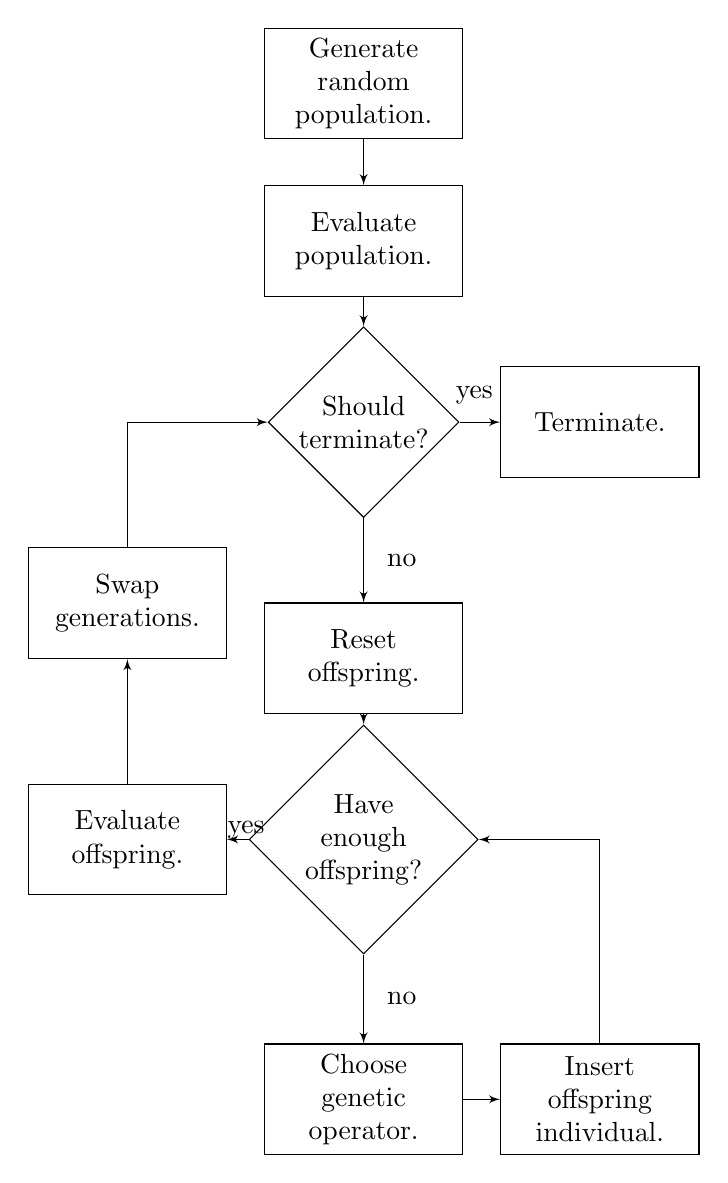
\begin{tikzpicture}[
				node distance = 2cm, 
				auto,
				decision/.style={
					diamond, 
					draw, 
		    		text width=5em, 
		    		text badly centered, 
		    		node distance=2.3cm, 
		    		inner sep=0pt
		    		},
				block/.style={
					rectangle, 
					draw, 
					text width=6.5em, 
					text centered, 
					minimum height=4em
					},
				line/.style={
					draw,
					-latex'
					}]
			    % Place nodes
			    \node [block] (init) {Generate random population.};
			    \node [block, below of=init] (evaluate2) {Evaluate\\population.};
			    \node [decision, below of=evaluate2] (termination) {Should terminate?};
			    \node [block, below of=termination, node distance=3cm] (reset) {Reset\\offspring.};
			    \node [block, right of=termination, node distance=3cm] (stop) {Terminate.};
			    \node [decision, below of=reset] (enough) {Have enough offspring?};

			    \node [block, below of=enough, node distance=3.3cm] (operator) {Choose genetic operator.};
			    \node [block, left of=enough, node distance=3cm] (evaluate) {Evaluate\\offspring.};
			    \node [block, above of=evaluate, node distance=3cm] (swap) {Swap\\generations.};
			    \node [block, right of=operator, node distance=3cm] (insert) {Insert\\offspring\\ individual.};

			    % Draw edges
			    \path [line] (init) -- (evaluate2);
			    \path [line] (evaluate2) -- (termination);
			    \path [line] (termination) -- node [xshift=5pt] {no}(reset);
			    \path [line] (reset) -- (enough);
			    \path [line] (enough) -- node [xshift=5pt] {no}(operator);
			    \path [line] (enough) -- node [xshift=3pt,yshift=10pt] {yes}(evaluate);
			    \path [line] (evaluate) -- (swap);
			    \path [line] (swap) |- (termination);
			    \path [line] (termination) -- node [xshift=-2pt,yshift=3pt] {yes}(stop);
			    \path [line] (operator) -- (insert);
			    \path [line] (insert) |- (enough);
			\end{tikzpicture}
		}
	\end{center}
\end{posterbox}

\begin{posterbox}[name=intro-swift,column=0,below=intro-ga]{Swift Programming Language}
	The Swift programming language has been unveiled in 2014 by the Apple Corporation. Since then, it has been widely adopted by software developers and computer engineers, succeeding Objective-C as the main programming language used for application development on the Apple mobile device platform. Building on proven coding paradigms, such as generics and strongly-typed objects, Swift strives to be a modern, concise and safe alternative to popular languages like Python or C++ while attempting to maintain comparable performance in terms of computational speed and memory management.
\end{posterbox}

\begin{posterbox}[name=arch,column=1]{Architecture}
	\todo
\end{posterbox}

\begin{posterbox}[name=props,column=1,below=arch]{Properties}
	\todo
\end{posterbox}

\begin{posterbox}[name=car,column=1,below=props]{Self-driving Car Simulation}
	The presented library was used to evolve a control program for a self-driving car. The environment assumed Newtonian physics model (ignoring friction forces) and the parameters of the experimental car were modelled to match a real vehicle. The road was a randomly generated closed Bézier curve, which was detectable by 5 sensors positioned in the front, middle and the back of the car (see the picture below).

	\vspace{0.5em}

	\parbox[c]{0.34\linewidth}{
		\resizebox{!} {3.2cm} {
			\begin{tikzpicture}[framed,background rectangle/.style={fill=black!60!green}]
				\draw[
				  black!10!white,
				  line width=3mm,
				  postaction={
				    decorate,
				    decoration={
				      markings,
				      mark=between positions 0 and 1 step 0.2 with
				      {
				        \node[transform shape] {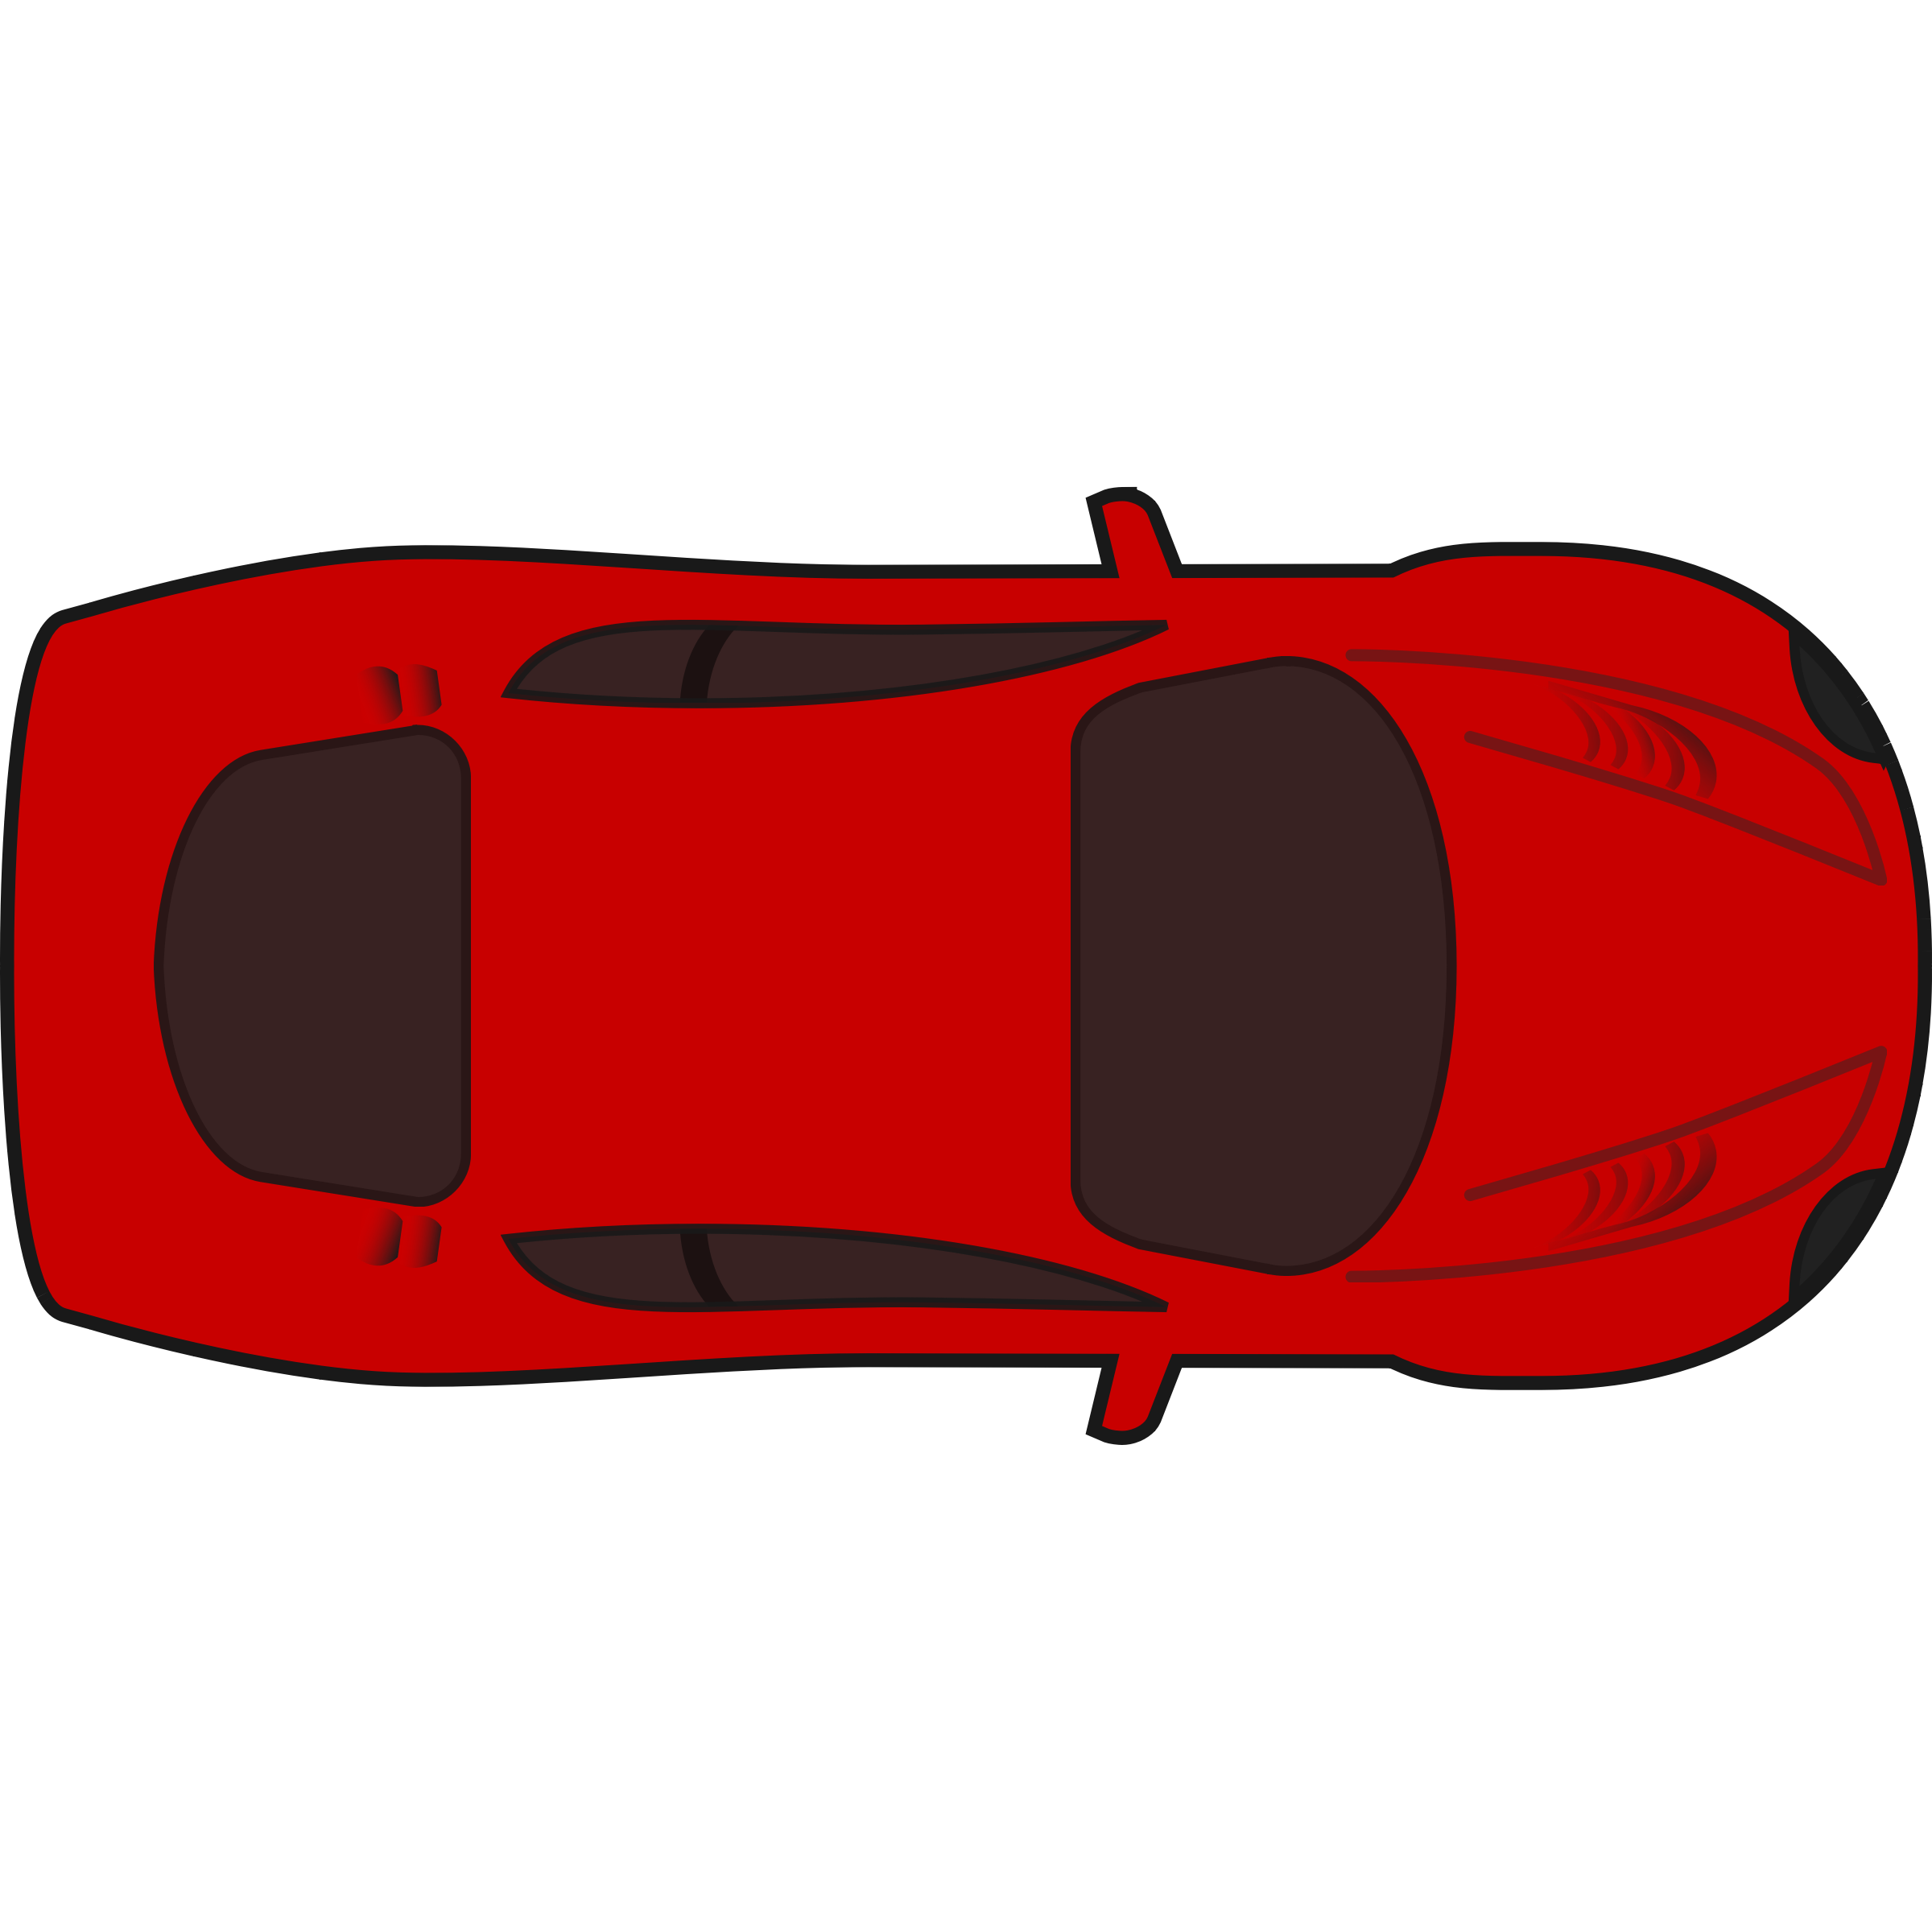
\includegraphics[width=.5cm]{car}};
				      }
				    }
				  }
				]
				(0,0) to[out angle=0,in angle=180,curve through={(1,.4) .. (5,0) .. (10,.5) .. (7,4.3) .. (3,4) .. (1,2)}] (0,0);
			\end{tikzpicture}
		}
	}
	\hfill
	\parbox[c]{0.24\linewidth}{
		\resizebox{!} {3.2cm} {
			\begin{tikzpicture}[detector/.style={draw,fill=yellow!70!white,minimum size=0.4cm,font=\bf}]
				\node[anchor=south west,inner sep=0,rotate=90] at (0,0) {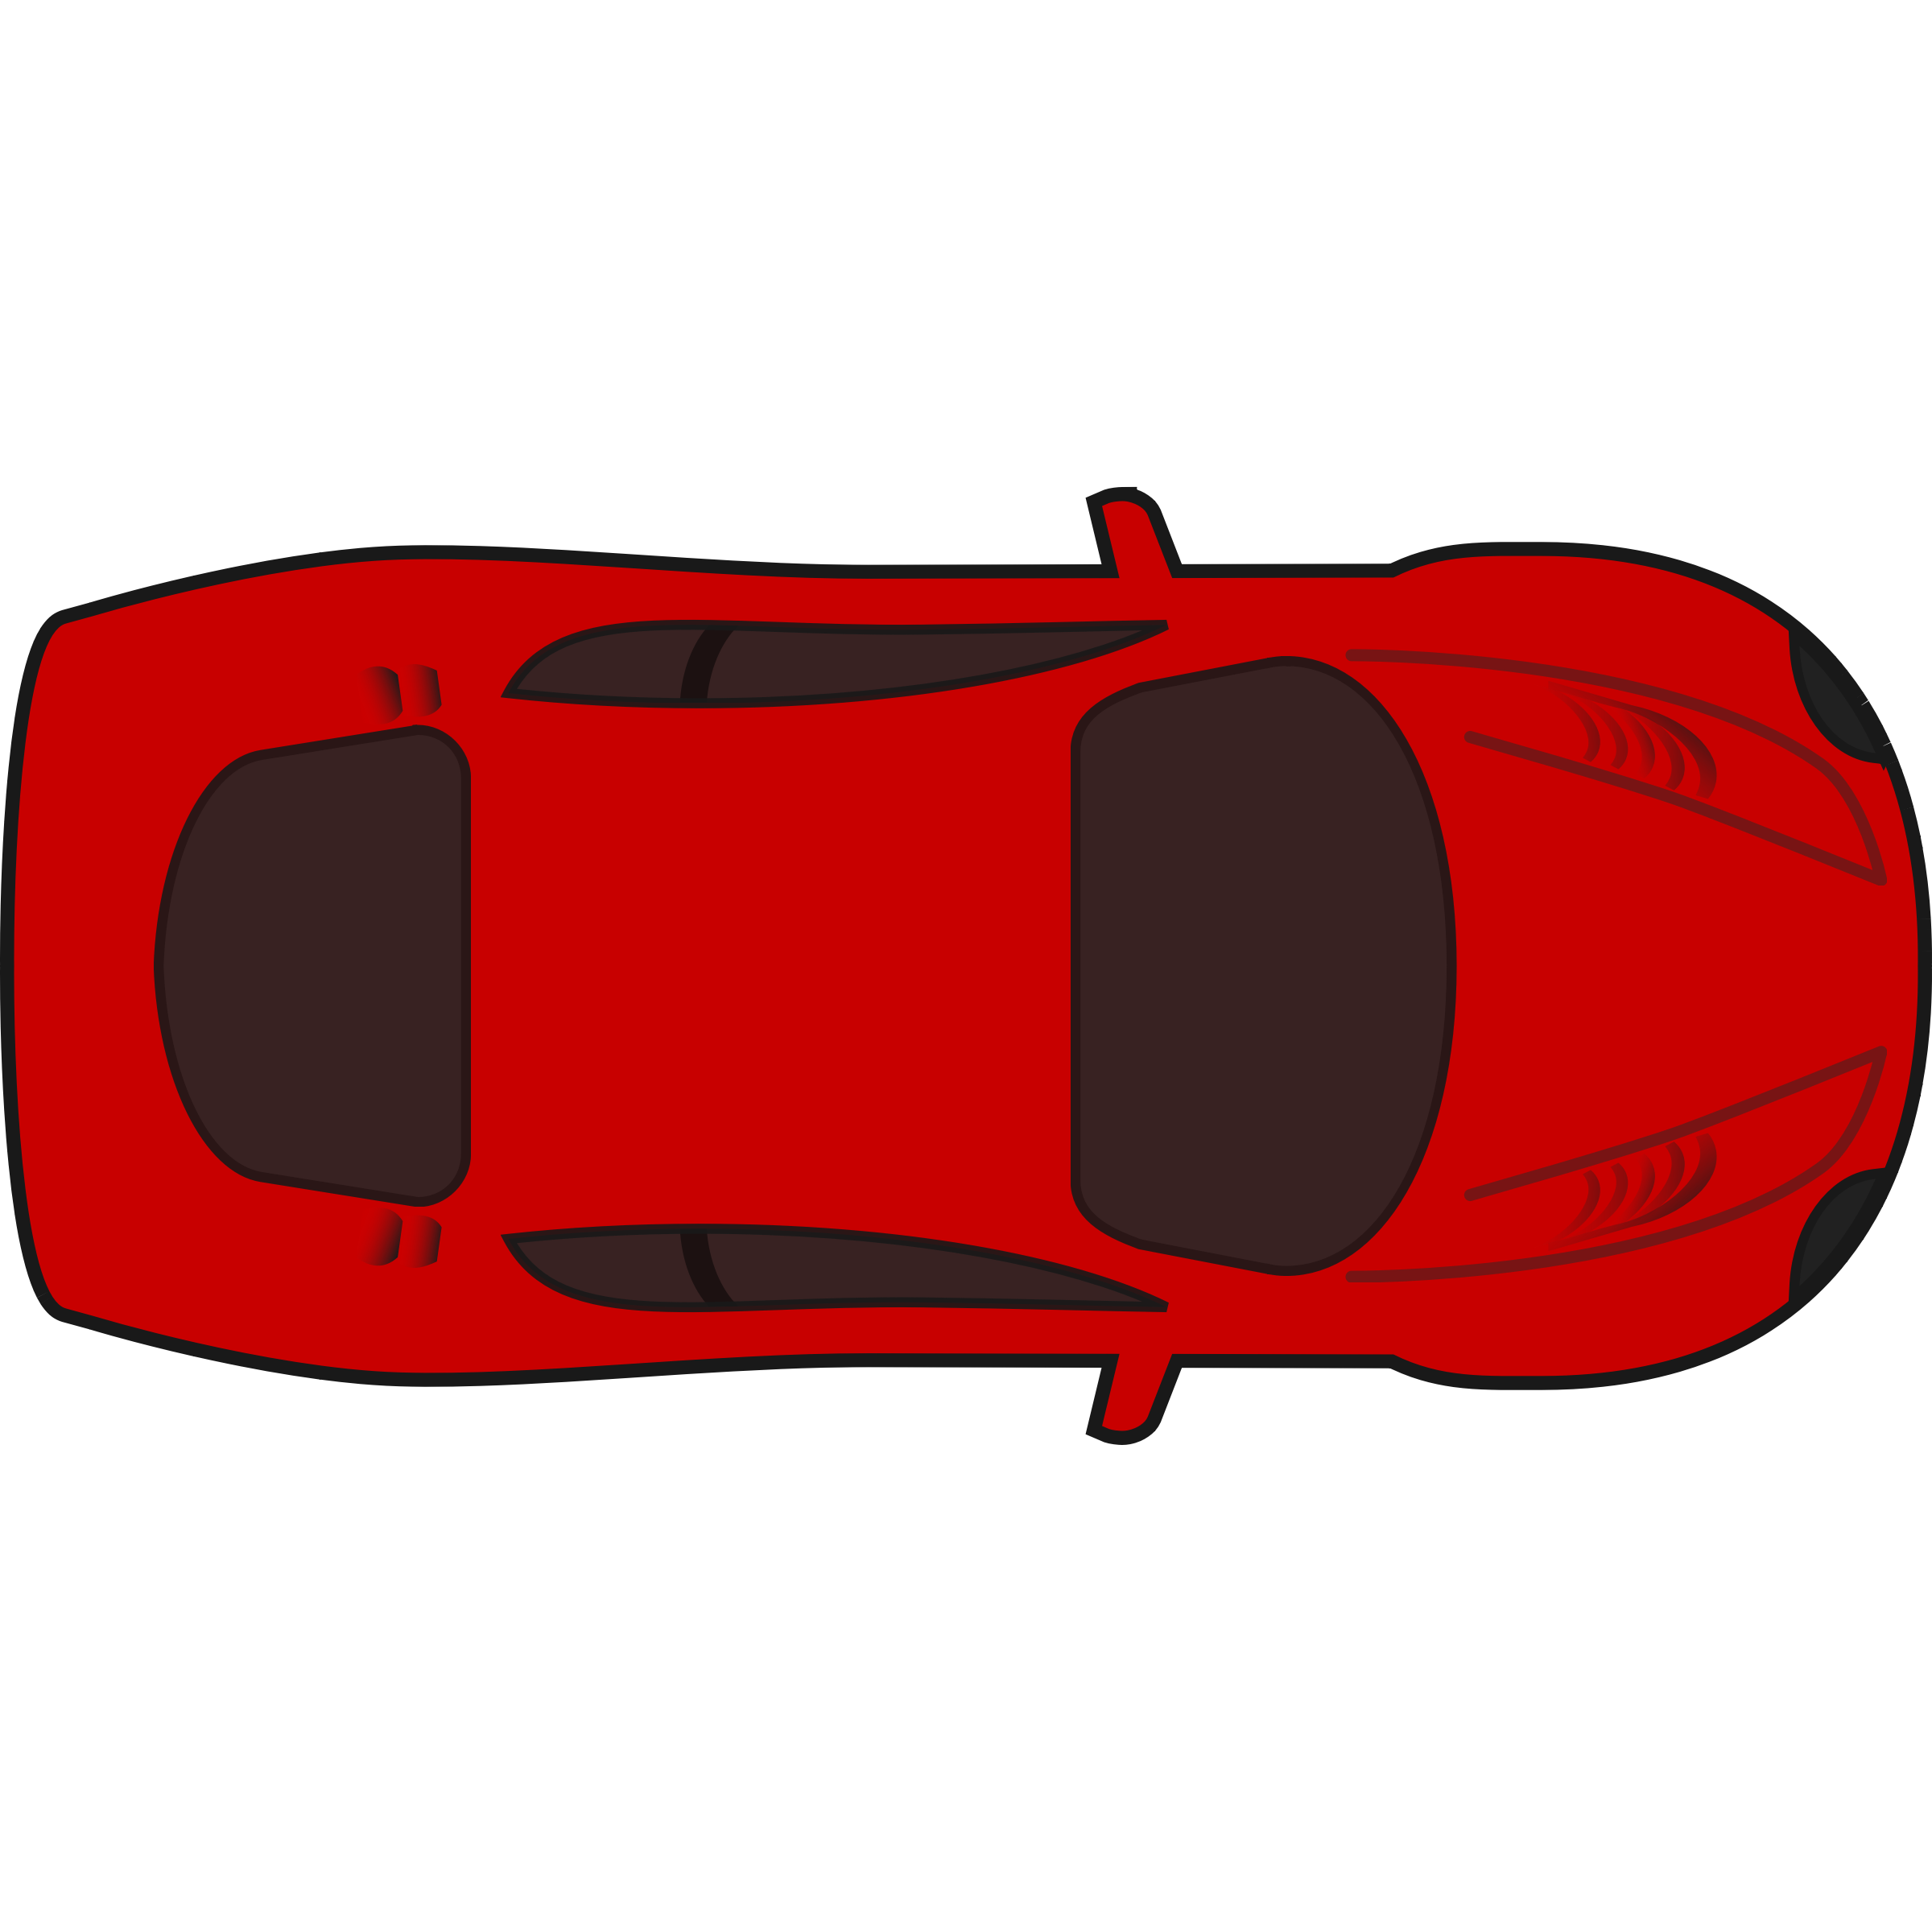
\includegraphics[width=2.8cm]{car}};
				\node[detector] at (-2,3.2) {1};
				\node[detector] at (-1.4,3.2) {2};
				\node[detector] at (-0.8,3.2) {3};
				\node[detector] at (-1.4,1.1) {4};
				\node[detector] at (-1.4,-0.7) {5};
			\end{tikzpicture}
		}
	}

	\vspace{0.5em}

	The car was controlled by a 3-layer feedforward neural network with 10 neurons in the hidden layer, whose connection weights were encoded in the genotype. Every program was evaluated in 5 independent 1-hour simulations, which tracked the total distance driven over the road. The fitness function was defined as

	\vspace{-1.7em}

	\begin{align*}
		f(\hat{d}_1,\hat{d}_2,\dots,\hat{d}_5) = \frac{1}{5 d_{max}} \sum_{i=1}^5 \hat{d}_i
	\end{align*}

	\vspace{-0.5em}

	where $\hat{d}_1,\hat{d}_2,\dots,\hat{d}_5$ denote the total distances driven over the road in the individual simulations and $d_{max}$ denotes the maximum achievable distance given the simulation parameters. The best control program after 100 generations was able to stay on the road in approximately 70\% of simulations.
	\vspace{-1.4em}

	\begin{center}
		\resizebox {\columnwidth} {!} {
			\begin{tikzpicture}
				\begin{axis}[
					height=6cm,
					width=9cm,
					grid=major,
					xlabel={Generation},
					ymin=0, ymax=1,
					xmin=1, xmax=100,
					no markers,
					legend style={legend pos=south east,font=\small},
			        yticklabel style={font=\small,xshift=-0.4ex},
			        xticklabel style={font=\small,yshift=-0.5ex},
			        xlabel style={font=\small,xshift=1.0ex}
				]
			
				\addplot table {data/car-fitness-best.dat};
				\addlegendentry{Best fitness}

				\addplot table {data/car-fitness-average.dat};
				\addlegendentry{Average fitness}

				\end{axis}
			\end{tikzpicture}
		}
	\end{center}
\end{posterbox}

\begin{posterbox}[name=qwop,column=2]{QWOP Player}
	QWOP is a popular online game, in which the player drives an athlete to finish a 100-meter sprint race as fast as possible. QWOP's difficulty is caused by its control scheme, which only allows the player to move the athlete by contracting individual muscle groups within his body. The challenge of the game is in that sense comparable to the problem of evolving bipedal gaits in physical robots.

	\vspace{0.5em}

	\parbox[c]{0.49\linewidth}{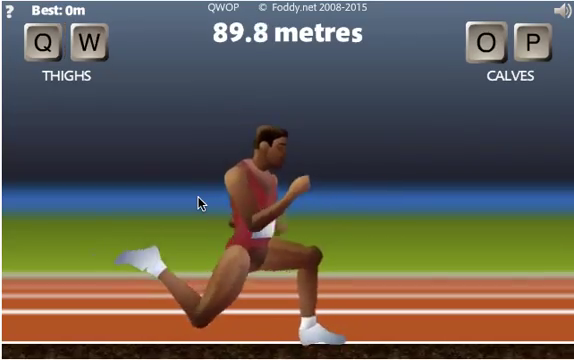
\includegraphics[width=\linewidth]{runner1}}
	\hfill
	\parbox[c]{0.49\linewidth}{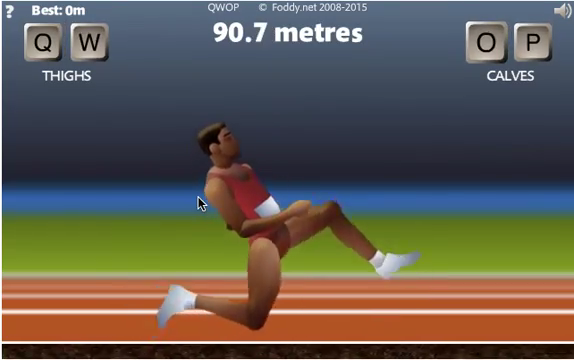
\includegraphics[width=\linewidth]{runner2}}

	\vspace{0.5em}

	The presented library was used to evolve an artificial QWOP player and partially replicate human-competitive results achieved by \todo. In every generation, 80 game strategies were generated and encoded as simple programs (genotype strings), then evaluated by the fitness function

	\vspace{-1.7em}

	\begin{align*}
		f(d_1,d_2,\dots,d_n) = \frac{1}{100n} \sum_{i=1}^n d_i
	\end{align*}

	\vspace{-0.5em}

	where $d_1,d_2,\dots,d_n$ denote the distances achieved in $n$ trial 30-second runs. The best strategy after 38 generations was able to complete the race in approximately 152 seconds.

	\vspace{-1.4em}

	\begin{center}
		\resizebox {\columnwidth} {!} {
			\begin{tikzpicture}
				\begin{axis}[
					height=5cm,
					width=9cm,
					grid=major,
					xlabel={Generation},
					ymin=0, ymax=0.3,
					xmin=1, xmax=38,
					no markers,
					legend style={legend pos=north west,font=\small},
					xtick={0,5,10,15,20,25,30,35,38},
					ytick={0,0.1,0.2,...,0.3},
			        yticklabel style={font=\small,xshift=-0.4ex},
			        xticklabel style={font=\small,yshift=-0.5ex},
			        xlabel style={font=\small,xshift=1.0ex}
				]
					
				\addplot table {data/qwop-fitness-best.dat};
				\addlegendentry{Best fitness}

				\addplot table {data/qwop-fitness-average.dat};
				\addlegendentry{Average fitness}

				\end{axis}
			\end{tikzpicture}
		}
	\end{center}
\end{posterbox}

\begin{posterbox}[name=conclusion,column=2,below=qwop]{Conclusions}
	This thesis has managed to satisfy all of its objectives. The presented library is available online as an open-source project and has many potential applications.
\end{posterbox}

\begin{posterbox}[name=ref,column=2,below=conclusion]{References}
	\todo
\end{posterbox}

\end{poster}
\end{document}
